\appendix 

\section{Additional examples.}
\label{sec:app:examples}

Figure~\ref{fig:tg_inter} shows the result of temporal intersection
of \insql{T1} with \insql{T2}.  Only the vertices and edges present in
both \tgs are produced, thus eliminating $v_3$ and $v_4$.  Period
$[2/15, 4/15)$ for $v_2$ is computed as a result of the join of
$[2/15, 5/15)$ in \insql{T1} and [$2/15, 4/15)$ in \insql{T2}.

Figure~\ref{fig:tg_diff} shows the result of temporal difference
of \insql{T1} with \insql{T2}.  Vertex v1 is removed between 2/15 and
6/15, splitting one v1 tuple in \tv of T1 into two temporally-disjoint
tuples in the result.

\begin{figure}[b]
\centering
\begin{subfigure}{3in}
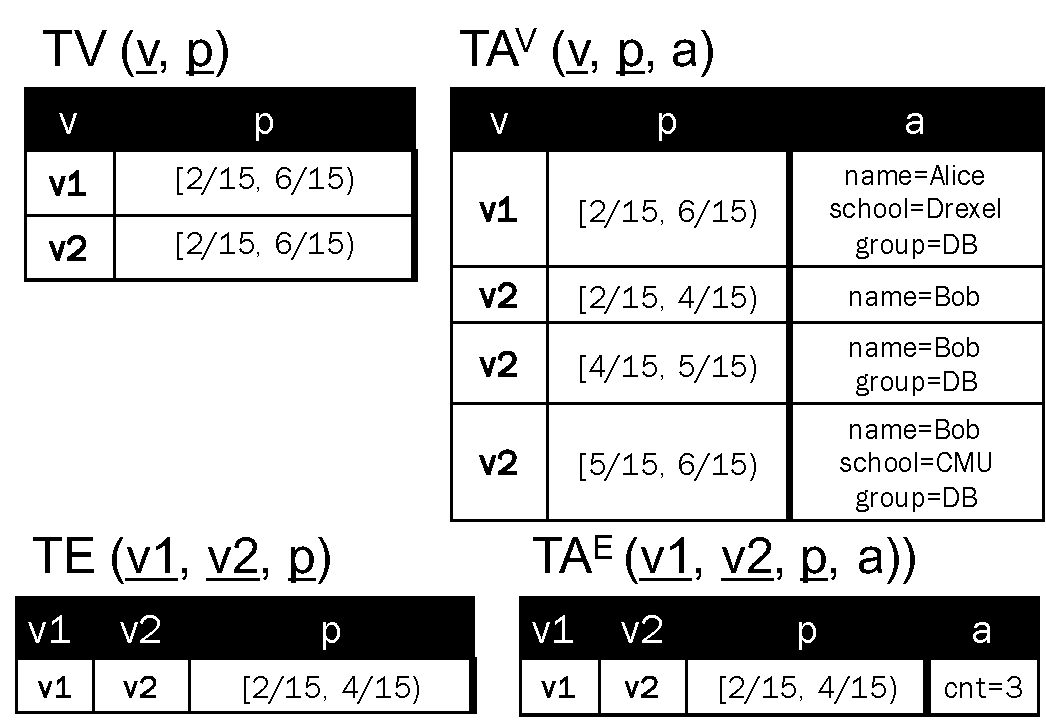
\includegraphics[width=2.8in]{figs/T1_inter_T2_rel.pdf}
\caption{$T1 \cap^T T2$.}
%\vspace{-0.2cm}
\label{fig:tg_inter}
\end{subfigure}
\begin{subfigure}{3in}
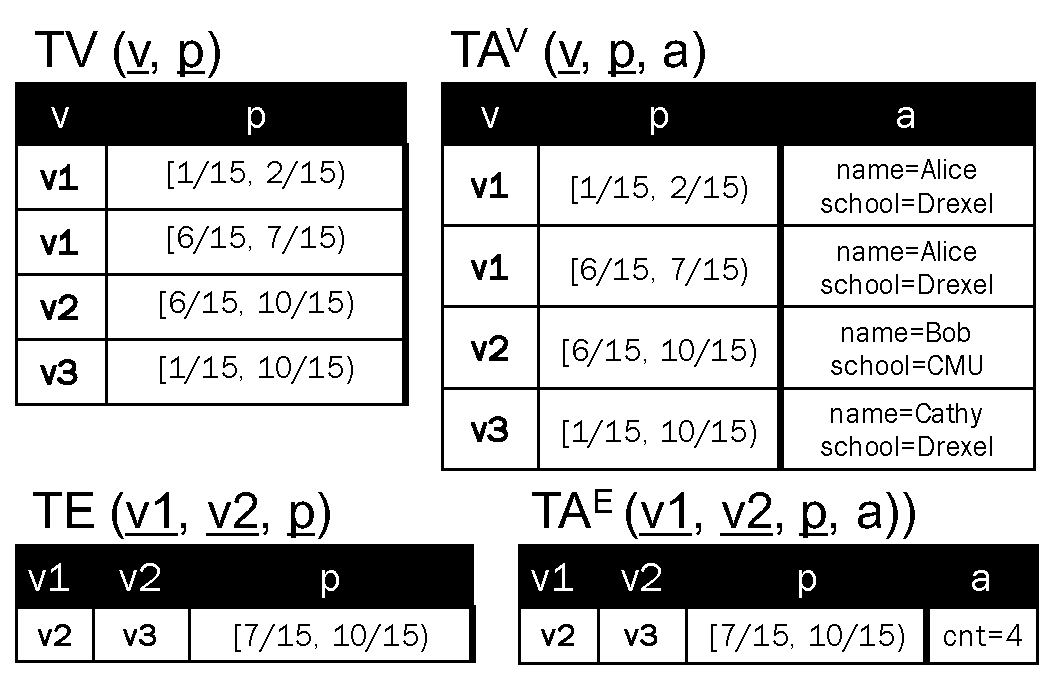
\includegraphics[width=2.8in]{figs/T1_diff_T2_rel.pdf}
\caption{$T1 \setminus^T T2$.}
\vspace{-0.2cm}
\label{fig:tg_diff}
\end{subfigure}
\caption{Binary operators.}
\label{fig:binary}
\vspace{-0.2cm}
\end{figure}


\section{Additional results.}
\label{sec:app2}

\begin{figure*}
%\centering
\begin{minipage}[b]{2.2in}
\centering
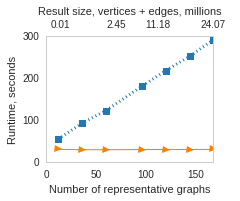
\includegraphics[width=2.1in]{figs/slice_wikitalk_build13.png}
\caption{Slice on wiki-talk.}
\label{fig:slicewiki}
\end{minipage}
\begin{minipage}[b]{2.2in}
\centering
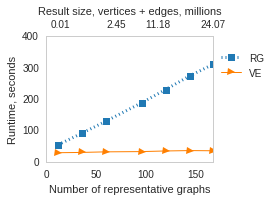
\includegraphics[width=2.1in]{figs/project_wikitalk_build13.png}
\caption{Map on wiki-talk.}
\label{fig:project}
\end{minipage}
\begin{minipage}[b]{2.2in}
\centering
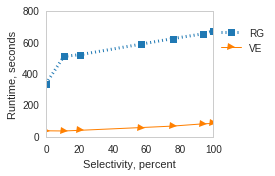
\includegraphics[width=2.4in]{figs/subgraph_wikitalk_build13.png}
\caption{Subgraph on wiki-talk.}
\label{fig:subgraphwiki}
\end{minipage}
\end{figure*}

\begin{figure*}
\centering
\begin{minipage}[b]{2in}
\centering
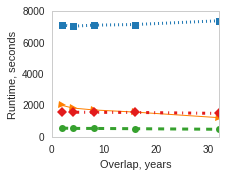
\includegraphics[width=2in]{figs/union_ngrams_build13.png}
\caption{Union on nGrams.}
\label{fig:union2}
\end{minipage}
\begin{minipage}[b]{2.3in}
\centering
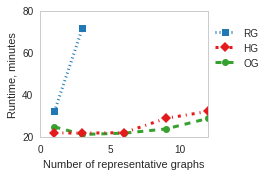
\includegraphics[width=2.3in]{figs/prank_twitter_build13.png}
\caption{PageRank on Twitter.}
\label{fig:pranktwitter}
\end{minipage}
\begin{minipage}[b]{2.3in}
\centering
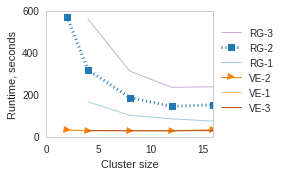
\includegraphics[width=2.3in]{figs/slice_wikitalk_scale_build13.png}
\caption{Scaling slice on wiki-talk.}
\label{fig:slicescale}
\end{minipage}
\end{figure*}

\begin{figure*}
\centering
\begin{minipage}{2.4in}
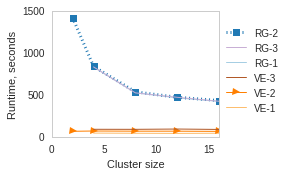
\includegraphics[width=2.4in]{figs/select_wikitalk_scale_build13.png}
%\vspace{-0.2in}
\caption{V-subgraph on wiki-talk.}
\label{fig:selectscale}
\end{minipage}
\end{figure*}

Plots and discussion in this section complement experimental results
presented in Section~\ref{sec:exp}.

Figure~\ref{fig:slicewiki} shows performance of VE and \sg
on \insql{slice} over wiki-talk.  It exhibits the same trend as on the
nGrams dataset in Figure~\ref{fig:slicengrams} but on a smaller scale.

Figure~\ref{fig:subgraphwiki} shows performance of VE and \sg
on \insql{vertex subgraph} over wiki-talk.  Wiki-talk dataset is small
enough that broadcast join can be used for constraining the edges, so
the sudden worsening of performance is not observed, as it is in
Figure~\ref{fig:subgraphngrams}.

We next examine how the different access methods scale with the size
of the cluster.  We varied the number of cluster workers while
executing individual operations.

To examine the performance on slice, we fixed the slice interval size
to be 4, 8, and 14 years (series -1, -2, and -3, respectively).  As
can be seen in Figure~\ref{fig:slicescale}, the performance of VE did
not change with the cluster size or the size of the interval.  Our
cluster stores the graph files on HDFS with no replication, and Spark
does not currently support filter pushdown on dates (this is being
addressed in one of the upcoming releases), so these results are
expected as the operation is essentially just a file scan.  \rg
performance did improve as the cluster grew, with the biggest
reduction occurring by 8 slaves and diminishing returns thereafter. 

Similar trends can be seen on vertex subgraph in
Figure~\ref{fig:selectscale}, where we fixed the query selectivity to
be 20, 57, and 100\%.  There is no observable difference between
different selectivity for \rg, which is consistent with the subgraph
experiment results.

We do not include results for every operation here as they all show
the same trends -- performance rapidly improves with increased cluster
size up to a point and adding additional slaves is not beneficial
thereafter.  \eat{The final result in Figure~\ref{fig:ccscale} shows
  the performance on connected components analytic with 2, 5, and 8
  years.  The very small cluster sizes led to executions that were
  stopped due to taking too long.}

\eat{For analytics, which are most computationally and
network traffic expensive, small cluster sizes lead to failed runs
with out of memory errors (this is a persistent problem in Spark
GraphX) or executions that were stopped due to taking longer than 2
hours.}

